\subsection{SMAR (model ID: 40)}
The SMAR model (fig.~\ref{fig:40_schematic}) is the result of a series of modifications to the original 'layers-model' \citep{OConnell1970} and summarized by \citet{Tan1996}. The model uses an arbitrary number of soil moistures stores connected in series, with each store having a depth of 25mm. The number of stores is an optimization parameter. The current storage in the upper 5 stores features in various equations. For consistency within this framework, the process is reversed: the model uses a fixed number of 5 soil moisture stores, but the depth of each store is variable and given as $S_{n,max} = S_{max} / 5$. It has 6 stores and 8 parameters ($H$, $Y$, $S_{max}$, $C$, $G$, $K_G$, $N$ and $K$). The model aims to represent:

\begin{itemizecompact}
\item Saturation excess overland flow;
\item Infiltration excess overland flow;
\item Gradual infiltration into soil moisture and declining evaporation potential when water is sourced from further underground;
\item Groundwater flow;
\item Routing of non-groundwater flow.
\end{itemizecompact}

\subsubsection{File names}
\begin{tabular}{@{}ll}
Model: &m\_40\_smar\_8p\_6s \\
Parameter ranges: &m\_40\_smar\_8p\_6s\_parameter\_ ranges \\
\end{tabular}

% Equations
\subsubsection{Model equations}

% Model layout figure
{ 																	% This ensures it doesn't warp text further down
\begin{wrapfigure}{l}{5cm}
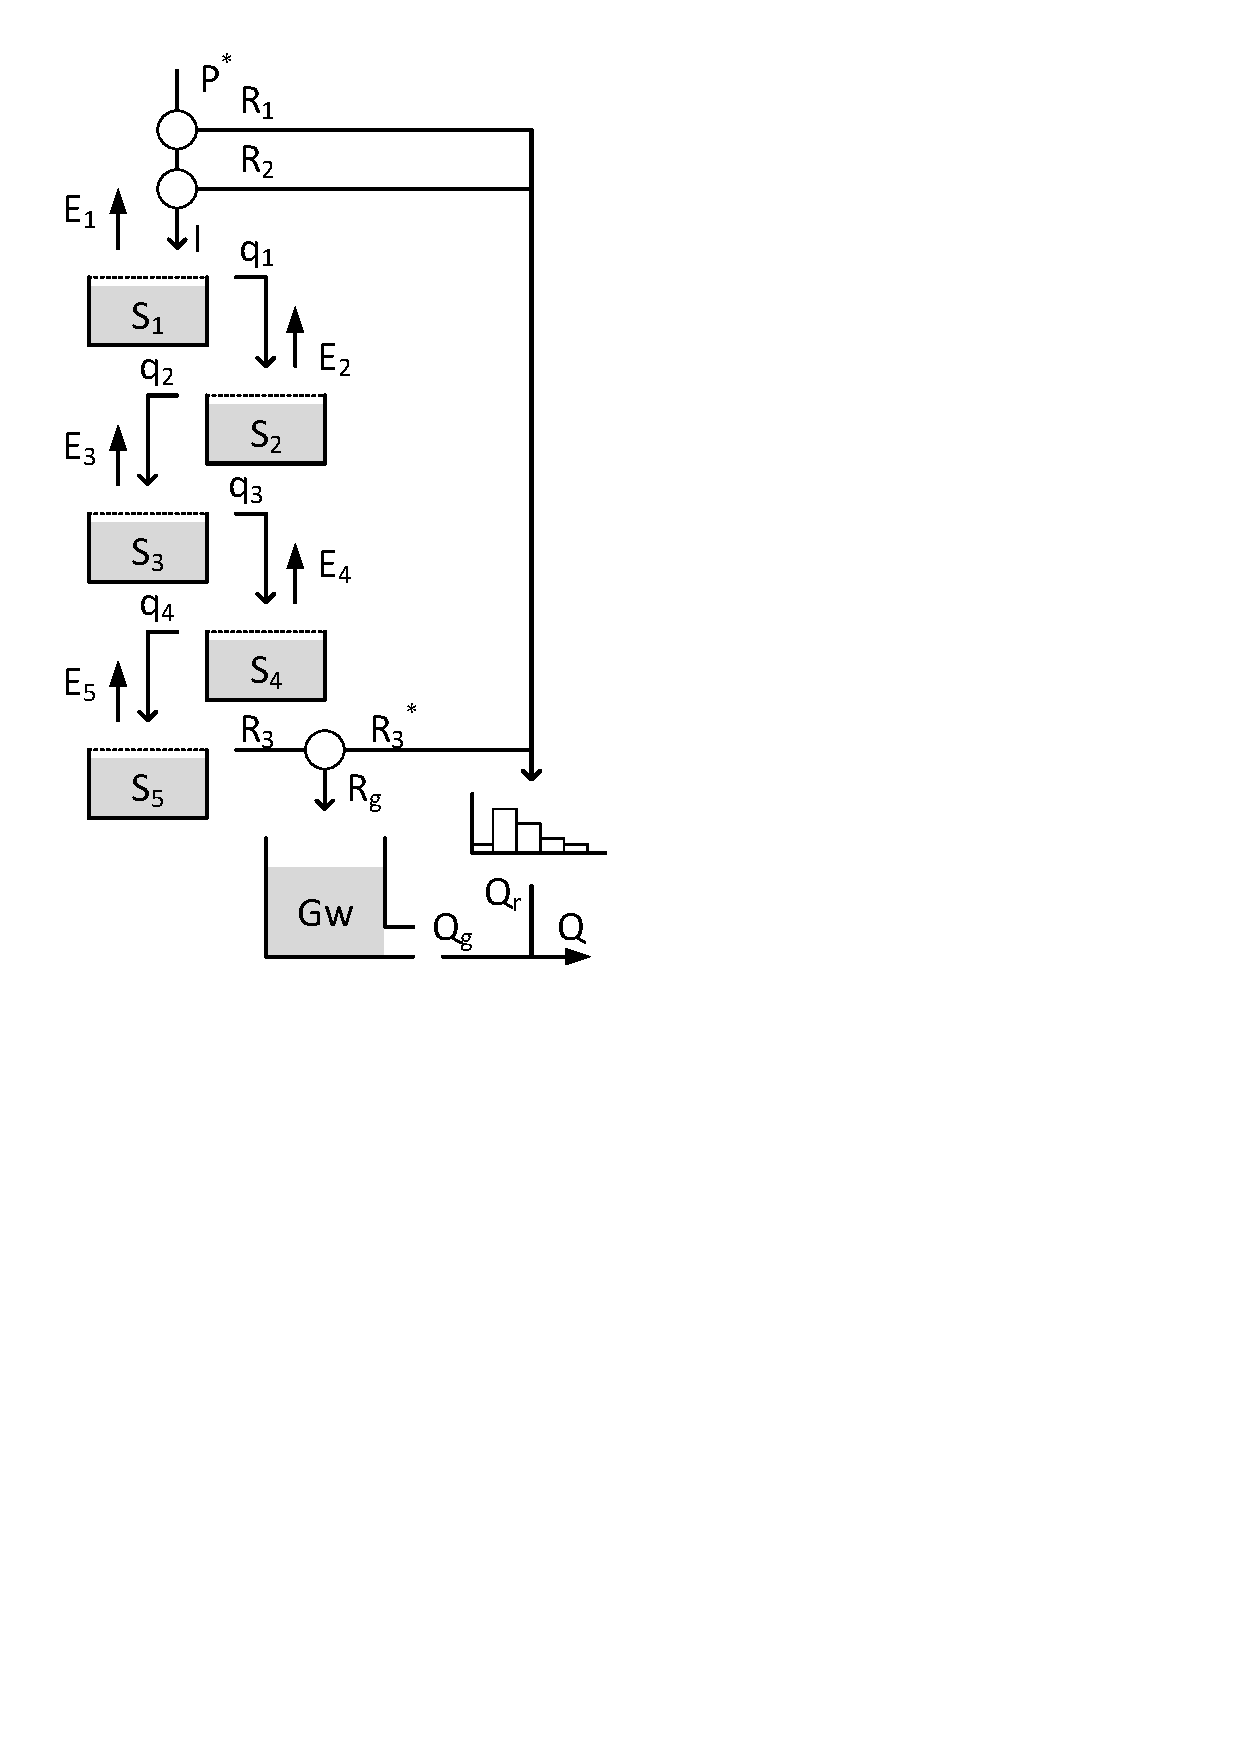
\includegraphics[trim=1cm 13cm 7cm 1cm,width=7cm,keepaspectratio]{./files/40_schematic.pdf}
\caption{Structure of the SMAR model} \label{fig:40_schematic}
\end{wrapfigure}

\begin{align}
	\frac{dS_1}{dt} &= I-E_1-q_1 \\
	I &= \begin{cases}
		Y, &\text{if } P^*-R_1 \geq Y \\
		P^*-R_1, & \text{otherwise} \\
		\end{cases}\\
	P^* &= \begin{cases}
		P-E_p, &\text{if } P > E_p \\
		0, & \text{otherwise} \\
	\end{cases} \\
	R_1 &= P^**H*\frac{\sum{S_n}}{S_{max}}\\
	R_2 &= \left(P^*-R_1\right) - I\\
	E_1 &= C^{(1-1)}*Ep^* \\
	E_p^* &= \begin{cases}
		E_p-P, &\text{if } E_p > P \\
		0, & \text{otherwise} \\
	\end{cases} \\
	q_1 &= 
	\begin{cases}
		P^*-R_1-R_2, & \text{if } S_1 \geq \frac{S_{max}}{5} \\
		0, & \text{otherwise}
	\end{cases}
\end{align}

} %end wrap figure

Where $S_1$ [mm] is the current storage in the upper soil layer, $I$ $[mm/d]$ infiltration into the soil, $P^*$ the effective precipitation $[mm/d]$, $R_1$ $[mm/d]$ is direct runoff, $R_2$ $[mm/d]$ is infiltration excess runoff, $E_1$ $[mm/d]$ evaporation and $q_1$ $[mm/d]$ flow towards deeper soil layers. $I$ uses a constant infiltration rate $Y$ $[mm/d]$. Direct runoff $R_1$ relies on distribution parameter $H$ [-] and is scaled by the current soil moisture storage in all layers compared to the maximum soil moisture storage $S_{max}$ [mm] of all layers. Evaporation from this soil layer occurs at the effect potential rate $E_p^*$. Runoff to deeper layers $q_1$ only occurs when the current storage exceeds the store's maximum capacity. 

\begin{align}
	S_2 &= q_1 - E_2 - q_2\\
	E_2 &= 
		\begin{cases}
		C^{(2-1)}*Ep , & \text{if } S_1 = 0\\
		0, & \text{otherwise}\\
	\end{cases}\\
	q_2 &= 
	\begin{cases}
		q1, & \text{if } S_2 \geq \frac{S_{max}}{5} \\
		0, & \text{otherwise}
	\end{cases}
\end{align}

Where $S_2$ [mm] is the current storage in the second soil layer, $E_2$ $[mm/d]$ the evaporation scaled by parameter $C$ [-], and $q_2$ $[mm/d]$ overflow into the next layer. Evaporation is assumed to occur only when the storage in the upper layers has been exhausted.

\begin{align}
	S_3 &= q_2 - E_3 - q_3\\
	E_3 &= 
		\begin{cases}
		C^{(3-1)}*Ep , & \text{if } S_2 = 0\\
		0, & \text{otherwise}\\
	\end{cases}\\
	q_3 &= 
	\begin{cases}
		q2, & \text{if } S_3 \geq \frac{S_{max}}{5} \\
		0, & \text{otherwise}
	\end{cases}
\end{align}

Where $S_3$ [mm] is the current storage in the second soil layer, $E_3$ $[mm/d]$ the evaporation scaled by parameter $C^2$ [-], and $q_3$ $[mm/d]$ overflow into the next layer. Evaporation is assumed to occur only when the storage in the upper layers has been exhausted.

\begin{align}
	S_4 &= q_3 - E_4 - q_4\\
	E_4 &= 
		\begin{cases}
		C^{(4-1)}*Ep , & \text{if } S_3 = 0\\
		0, & \text{otherwise}\\
	\end{cases}\\
	q_4 &= 
	\begin{cases}
		q3, & \text{if } S_4 \geq \frac{S_{max}}{5} \\
		0, & \text{otherwise}
	\end{cases}
\end{align}

Where $S_4$ [mm] is the current storage in the second soil layer, $E_4$ $[mm/d]$ the evaporation scaled by parameter $C^3$ [-], and $q_4$ $[mm/d]$ overflow into the next layer. Evaporation is assumed to occur only when the storage in the upper layers has been exhausted.

\begin{align}
	S_5 &= q_4 - E_5 - R_3\\
	E_5 &= 
		\begin{cases}
		C^{(5-1)}*Ep , & \text{if } S_4 = 0\\
		0, & \text{otherwise}\\
	\end{cases}\\
	R_3 &= 
	\begin{cases}
		q4, & \text{if } S_5 \geq \frac{S_{max}}{5} \\
		0, & \text{otherwise}
	\end{cases}
\end{align}

Where $S_5$ [mm] is the current storage in the second soil layer, $E_5$ $[mm/d]$ the evaporation scaled by parameter $C^4$ [-], and $R_3$ $[mm/d]$ overflow towards groundwater. Evaporation is assumed to occur only when the storage in the upper layers has been exhausted.

\begin{align}
	\frac{dG_w}{dt} &= R_g -Q_g\\
	R_g &= G*R_3\\
	Q_g &= K_G*G_w
\end{align}

Where $ G_w$ [mm] is the current groundwater storage, refilled by fraction $G$ [-] of $R_3$ $[mm/d]$ and drained as a linear reservoir with time parameter $K_G$ $[d^{-1}]$. This groundwater flow $Q_g$   $[mm/d]$ contributes directly to simulated streamflow $Q$. The fraction $R_3^* = (1-G)*R_3$ that does not reach the groundwater reservoir is combined with $R_1$ and $R_2$ and routed with a gamma function with parameters $N$ and $K$. The routing function approximates a Nash-cascade consisting of $N$ reservoirs with storage coefficient $K$ [d]: 

\begin{align}
 	Q_r &= \left(R_1+R_2+R_3\right)\frac{1}{K\Gamma(N)}\left(\frac{t}{K}\right)^{N-1}e^{-t/K}
\end{align}

Integration over the time step length $d$ provides the fraction of flow routed per time step $Q_r$ $[mm/d]$. Total flow:

\begin{align}
	Q_t = Q_r+Q_g
\end{align}

\newpage
\subsubsection{Parameter overview}
% Table generated by Excel2LaTeX from sheet 'Sheet1'
\begin{table}[htbp]
  \centering
    \begin{tabular}{lll}
    \toprule
    Parameter & Unit  & Description \\
    \midrule
    $H$   & $-$   & Fraction of effective precipitation that is direct runoff \\
    $Y$   & $mm~d^{-1}$ & Infiltration rate \\
    $S_{max}$ & $mm$  & Maximum soil moisture storage \\
    $C$   & $-$   & Evaporation reduction parameter \\
    $G$   & $-$   & Fraction of subsurface flow to groundwater \\
    $K_G$ & $d^{-1}$ & Runoff coefficient \\
    $N$   & $-$   & Gamma function parameter \\
    $K$   & $d$   & Routing time parameter \\
    \bottomrule
    \end{tabular}%
  \label{tab:addlabel}%
\end{table}%
